%%%%%%%%%%%%%%%%%%%%%%%%%%%%%%%%%%%%%%%%%
% Short Sectioned Assignment LaTeX Template Version 1.0 (5/5/12)
% This template has been downloaded from: http://www.LaTeXTemplates.com
% Original author:  Frits Wenneker (http://www.howtotex.com)
% License: CC BY-NC-SA 3.0 (http://creativecommons.org/licenses/by-nc-sa/3.0/)
%%%%%%%%%%%%%%%%%%%%%%%%%%%%%%%%%%%%%%%%%

% \documentclass[paper=a4, fontsize=11pt]{scrartcl} % A4 paper and 11pt font size
\documentclass[11pt, a4paper]{book}
\usepackage[T1]{fontenc} % Use 8-bit encoding that has 256 glyphs
\usepackage[utf8]{inputenc}
\usepackage{fourier} % Use the Adobe Utopia font for the document - comment this line to return to the LaTeX default
\usepackage{listings} % para insertar código con formato similar al editor
\usepackage[spanish, es-tabla]{babel} % Selecciona el español para palabras introducidas automáticamente, p.ej. "septiembre" en la fecha y especifica que se use la palabra Tabla en vez de Cuadro
\usepackage{url} % ,href} %para incluir URLs e hipervínculos dentro del texto (aunque hay que instalar href)
\usepackage{graphics,graphicx, float} %para incluir imágenes y colocarlas
\usepackage[gen]{eurosym} %para incluir el símbolo del euro
\usepackage{cite} %para incluir citas del archivo <nombre>.bib
\usepackage{enumerate}
\usepackage{hyperref}
\usepackage{graphicx}
\usepackage{tabularx}
\usepackage{booktabs}

\usepackage[table,xcdraw]{xcolor}
\hypersetup{
	colorlinks=true,	% false: boxed links; true: colored links
	linkcolor=black,	% color of internal links
	urlcolor=cyan		% color of external links
}
\renewcommand{\familydefault}{\sfdefault}
\usepackage{fancyhdr} % Custom headers and footers
\pagestyle{fancyplain} % Makes all pages in the document conform to the custom headers and footers
\fancyhead[L]{} % Empty left header
\fancyhead[C]{} % Empty center header
\fancyhead[R]{Me Llamo Así} % My name
\fancyfoot[L]{} % Empty left footer
\fancyfoot[C]{} % Empty center footer
\fancyfoot[R]{\thepage} % Page numbering for right footer
%\renewcommand{\headrulewidth}{0pt} % Remove header underlines
\renewcommand{\footrulewidth}{0pt} % Remove footer underlines
\setlength{\headheight}{13.6pt} % Customize the height of the header

\usepackage{titlesec, blindtext, color}
\definecolor{gray75}{gray}{0.75}
\newcommand{\hsp}{\hspace{20pt}}
\titleformat{\chapter}[hang]{\Huge\bfseries}{\thechapter\hsp\textcolor{gray75}{|}\hsp}{0pt}{\Huge\bfseries}
\setcounter{secnumdepth}{4}
\usepackage[Lenny]{fncychap}


\begin{document}

	% Plantilla portada UGR
	\begin{titlepage}
\newlength{\centeroffset}
\setlength{\centeroffset}{-0.5\oddsidemargin}
\addtolength{\centeroffset}{0.5\evensidemargin}
\thispagestyle{empty}

\noindent\hspace*{\centeroffset}\begin{minipage}{\textwidth}

\centering

\includegraphics[width=0.9\textwidth]{logos/logo_ugr.jpg}\\[1.4cm]

\textsc{ \Large TRABAJO FIN DE GRADO\\[0.2cm]}
\textsc{ GRADO EN INGENIERIA INFORMATICA}\\[1cm]

{\Huge\bfseries Título \\}
\noindent\rule[-1ex]{\textwidth}{3pt}\\[3.5ex]
{\large\bfseries Subtítulo }
\end{minipage}

\vspace{2.5cm}
\noindent\hspace*{\centeroffset}
\begin{minipage}{\textwidth}
\centering

\textbf{Autor}\\ {Estudiante}\\[2.5ex]
\textbf{Director}\\ {Tutor(a)(es)}\\[2cm]

\includegraphics[width=0.3\textwidth]{logos/etsiit_logo.png}\\[0.1cm]
\textsc{Escuela Técnica Superior de Ingenierías Informática y de Telecomunicación}\\
\textsc{---}\\
Granada, Junio de 201x
\end{minipage}
\end{titlepage}


	% Plantilla prefacio UGR
	\thispagestyle{empty}

\begin{center}
{\large\bfseries Port de un sistema operativo de tiempo real a una placa ARM \\ FreeRTOS en ARM7TDMI-S }\\
\end{center}
\begin{center}
Enrique Paubert Reca\\
\end{center}

%\vspace{0.7cm}

\vspace{0.5cm}
\noindent\textbf{Palabras clave}: \textit{software libre}, \textit{sistema operativo de tiempo real}, \textit{RTOS}, \textit{tiempo real}, \textit{ARM}, \textit{sistemas embebidos}
\vspace{0.7cm}

\noindent\textbf{Resumen}\\
	

\cleardoublepage

\begin{center}
	{\large\bfseries Same, but in English}\\
\end{center}
\begin{center}
	Enrique Paubert Reca\\
\end{center}
\vspace{0.5cm}
\noindent\textbf{Keywords}: \textit{open source}, \textit{floss}
\vspace{0.7cm}

\noindent\textbf{Abstract}\\


\cleardoublepage

\thispagestyle{empty}

\noindent\rule[-1ex]{\textwidth}{2pt}\\[4.5ex]

D. \textbf{Tutora/e(s)}, Profesor(a) del ...

\vspace{0.5cm}

\textbf{Informo:}

\vspace{0.5cm}

Que el presente trabajo, titulado \textit{\textbf{Port de un sistema operativo de tiempo real a una placa ARM}},
ha sido realizado bajo mi supervisión por \textbf{Enrique Paubert Reca}, y autorizo la defensa de dicho trabajo ante el tribunal
que corresponda.

\vspace{0.5cm}

Y para que conste, expiden y firman el presente informe en Granada a Junio de 2024.

\vspace{1cm}

\textbf{El/la director(a)/es: }

\vspace{5cm}

\noindent \textbf{(nombre completo tutor/a/es)}

\chapter*{Agradecimientos}

A mis padres, por estar ahí a pesar de todo lo que ha costado.

A Juan Pedro, porque sin el no habría empezado esta carrera.

A Shei, porque sin ella no la habría terminado.






	% Índice de contenidos
	\newpage
	\tableofcontents

	% Índice de imágenes y tablas
	\newpage
	\listoffigures

	% Si hay suficientes se incluirá dicho índice
	\listoftables 
	\newpage

	% Introducción 
	\chapter{Introducción}

Este proyecto es software libre, y está liberado con la licencia \cite{gplv3}.

\section{Motivación}

La motivación de este Trabajo de Fin de Grado surgió tras cursar la asignatura de Sistemas Empotrados del grado. Sentí que, aunque habíamos trabajado muy bien la base de los sistemas con el mismo nombre, quería profundizar algo más porque es un tema que considero muy interesante. 

Además, durante los años de la carrera, había oído hablar de los sistemas operativos de tiempo real, que también llamaron mucho mi atención, de manera que he decidido trabajar estos dos intereses en este proyecto.  



Tras cursar la asignatura de Sistemas Empotrados sentí que quería profundizar en mi conocimiento de estos sistemas en mi trabajo de fin de grado. Además, durante el grado había oido hablar de sistemas de tiempo real, pero no había trabajado con ninguno. De manera que he juntado estos dos intereses en este proyecto.


\section{Estructura}
\begin{enumerate}
    \item \textbf{Introducción:} En este capítulo se aborda la motivación del proyecto y se describe la estructura del documento.
    \item \textbf{Descripción del problema:} Se detallan el objetivo del proyecto, las restricciones a considerar y los requisitos necesarios para llevarlo a cabo.
    \item \textbf{Antecedentes:} Se presenta el contexto tecnológico, definiciones y datos relevantes que permiten comprender el entorno de los sistemas empotrados y de tiempo real.
    \item \textbf{Estudio de requisitos:} En este apartado se describen los casos de uso, los requisitos y los actores que definen y limitan el alcance del proyecto.
    \item \textbf{Análisis del problema:} Se analizan las decisiones relacionadas con la elección de hardware y software para asegurar el correcto funcionamiento del sistema.
    \item \textbf{Planificación:} Se establece un cronograma para el proyecto y se discuten otros factores importantes como el presupuesto y las fases de implementación del mismo.
    \item \textbf{Implementación:} Se detalla el proceso de implementación del proyecto, siguiendo las fases definidas en la planificación y abordando los problemas encontrados en las diferentes etapas.
    \item \textbf{Conclusiones y trabajos futuros:} Este capítulo final ofrece una valoración del trabajo realizado, detalla los conocimientos adquiridos durante la realización de este proyecto y propone posibles líneas de trabajo futuras.
\end{enumerate}


	% Descripción del problema y hasta donde se llega
	\chapter{Descripción del problema}
\section{El problema}
En la actualidad existen multitud de placas diseñadas para sistemas embebidos, así como una gran cantidad de sistemas operativos y firmwares que se utilizan para facilitar el desarrollo de aplicaciones para las mismas.
Para muchas de estas aplicaciones modernas es útil o necesario el uso de sistemas de tiempo real, pues permite establecer restricciones de tiempo predecibles y consistentes, además de poder crear una planificación que se ajuste a nuestros objetivos.\\
El problema radica en la inmensa cantidad de placas que, aun teniendo los requisitos necesarios para el proyecto que tengamos entre manos, carecen de la posibilidad de utilizar un RTOS, perdiendo flexibilidad y aumentando los tiempos de desarrollo, y obligándonos a buscar opciones que no sean tan favorables.
Además los sistemas operativos de tiempo real prediminantemente utilizados en la industria son desarrollados por empresas que poseen software propietario, lo que dificulta el aprendizaje y el acceso a estos sistemas.

% En la actualidad, el uso de sistemas embebidos esta creciendo de manera exponencial en nuestra sociedad, así como la implementación de sistemas operativos de tiempo real (RTOS). Si bien estos últimos estan implementados en multitud de placas de sistemas empotrados, aún existe un gran número de placas que no tienen posibilidad de utilizar este RTOS, perdiendo la flexibilidad y la funcionalidad que estos podrian ofrecer.

\section{La solución}
Se propone la realización de una adaptación o \textit{port} de un sistema operativo de tiempo real a una placa ARM con el objetivo de aprender sobre la arquitectura de los sistemas operativos, las restricciones de el tiempo real 

% \itemize


	% Estado del arte
	% 	1. Crítica al estado del arte
	% 	2. Propuesta
	\chapter{Antecedentes}

\noindent\fbox{
	\parbox{\textwidth}{
    En este capítulo hablaré de el contexto actual en el que se desarrolla este projecto y daré algunas definiciones relevantes.
	}
}\\

El software libre y sus licencias \cite{gplv3} ha permitido llevar a cabo una expansión del aprendizaje de la informática sin precedentes.

\section{Descripción de la tecnología}
\subsection{Sistemas embebidos}
% NOTE: "ordenadores" o "sistemas informáticos"?
Cuando hablamos de ordenadores generalmente se piensa sobremesas o portátiles, y tal vez en teléfonos inteligentes, tablets o tal vez incluso servidores. A pesar de la ubicuidad de estos sistemas, muchos de los ordenadores con los que interactuamos a diario son invisibles, estan embebidos.

% \begin{center}\colorbox{cyan!10}{\fbox{ \begin{minipage}{11cm}
Los \Def{Sistemas Embebidos} son combinaiones de software y hardware (opcionalmente con partes mecánicas), de proposito específico y con un número reducido y definido de funciones. Pueden ser independientes o formar parte de otro sistema. Generalmente tienen una serie de restricciones como el uso de energía y capacidad para trabajar bajo condiciones adversas. Ejemplos: Lector de tarjetas de metro o autobús, TV, router, frigorífico, TPV, la multitud de sistemas que hay en un coche... \cite{es_glossary} \cite{marwedel}
% \end{minipage} }} \end{center}

% \begin{center}\colorbox{cyan!10}{\fbox{ \begin{minipage}{11cm}
En cambio, los \textbf{ordenadores de propósito general} es una combinación de hardware y software diseñados para un proposito general, es decir, sin un límite establecido de funiciones. Ejemplos: PC, teléfono inteligente, servidor... \cite{es_glossary}
% \end{minipage} }} \end{center}

Dos ejemplos claros de la diferencia entre un sistema empotrado y uno de proposito general serían la Nintendo Switch y la Steam Deck. La Nintendo Switch es un sistema empotrado, una consola diseñada para jugar a videojuegos que no tiene, por ejemplo, la función de navegar por internet por motivos de seguridad. La Steam Deck es un sistema con un factor de forma similar pero es un ordenador de proposito general que no ha sido limitado por diseño, aunque su principal proposito sea el de jugar a videojuegos.

% TODO: Insertar imágenes de Switch y Steam Deck aqui
%
%
%
%
%

\begin{center} \colorbox{yellow!10} { \fbox{ \begin{minipage}{11cm}
				Existe un debate sobre si teléfono o una tablet es un sistema empotrado, y con respecto a los \textit{dumbphones} o móviles no inteligentes es cierto dado que tienen un reducido número de funciones, pero mi opinión es que los móviles actuales se pueden utilizar como ordenadores de propósito general y la línea entre tablet y portátil se difumina cada vez más.
			\end{minipage} } } \end{center}

\subsubsection{BSPs}
Un \Def{Board Support Package} o BSP en el contexto de los sistemas empotrados es un \textit{firmware} diseñado para un hardware concreto que proporciona una secuencia de arranque y drivers para los dispositivos de la placa, entre otras funciones.

\subsection{RISC}
\Def{RISC}

\subsection{ARM}
\Def{ARM}

\subsection{Computación en Tiempo Real}
Los sistemas de \Def{Tiempo Real} son un tipo de sistema donde el funcionamiento correcto del mismo no depende solamente de que el resultado lógico sea correcto, sino también del tiempo requerido para llegar a ese resultado \cite{stankovic}. Esto no quiere decir necesariamente que las tareas deban tardar el mínimo tiempo posible, sino que el tiempo que se tarda en realizar una tarea debe de ser acotado, predecible y consistente.

Un ejemplo de como la consistencia se valora más que la velocidad es que en muchos sistemas de tiempo real no se utiliza memoria caché, ya que a pesar de que puede acelerar la computación, los aciertos y fallos de caché son difíciles de predecir y pueden provocar inconsistencias en el tiempo de ejecución \cite{MILLIGAN1996}.

La computación en tiempo real puede aplicarse tanto a ordenadores como sistemas empotrados y redes de comunicaciones. Algunos ejemplos incluyen sistemas de control de procesos, sistemas de conducción autónoma y sistemas de control de tráfico aéreo.

\subsubsection{Tiempo real «duro» y «blando»}
Cuando hablamos de sistemas de tiempo real existe la distinción entre sistemas de tiempo real «duros» (\textit{hard real time}) y «blandos» (\textit{soft real time}). \textit{Hard real time} se refiere a sistemas críticos donde una \textit{deadline} no cumplida puede tener resultados catastróficos, como puede ser en campos como la medicina o la aeroespacial. En cambio el \textit{soft real time} abarca problemas donde las \textit{deadline} no son tan estrictas y incumplirlas degradará la experiencia pero el sistema podrá seguir funcionando. Ejemplos de esto son el \textit{streaming} de elementos multimedia o la comunicación utilizando \textit{VoIP (Voice over IP)}. Mientras que el tiempo real «blando» se suele implementar dentro de otros sistemas que no requieren tiempo real, el tiempo real «duro» se implementa dentro de sistemas especialiados.

Dos ejemplos que muestran esta distinción son el ABS de un coche y una videoconsola. El ABS es un sistema de tiempo real «duro» ya que si no reacciona a tiempo puede provocar una colisión. En cambio una videoconsola es un sistema de tiempo real blando, debe realizar los cálculos necesarios para cada \textit{frame} del juego a tiempo de manera que se mantenga un \textit{framerate} estable, pero si se retrasa alguno se puede seguir jugando al juego.\\

Esta clasificación de «duro» y «blando» es más un espectro. Hay sistemas con mayores y menores tolerancias pero no existe una linea definida que separe claramente los sistemas de tiempo real «duros» y «blandos». Aun así la mayoría del trabajo de investigación que se realiza entorno al tiempo real se refiere a la parte del espectro que se considera tiempo real «duro».

También en este espectro existen el \textit{firm real time} que se refiere a sistemas donde, si no se alcanza una \textit{deadline}, el resultado de la operacion es irrelevante. Un ejemplo es un sistema que predice el tiempo, si el cálculo de la simulación es que va a llover pero ya ha empezado a llover el resultado no sirve para nada \cite{wang2017rtes}.

\subsubsection{Sistemas Operativos de Tiempo Real}
Los sistemas de tiempo real «duro» suelen utilizar sistemas operativos especializados llamados \Def{Sistemas operativos de tiempo real} (\textit{RTOS} por sus siglas en inglés). La diferencia más importante de los sistemas operativos de tiempo real con respecto a los de propósito general es la planificación. estos últimos utilizan \textit{FIFO}, \textit{Round-Robin} o colas con prioridad entre otros (o una combinación de varios) para planificar las tareas que el sistema o los usuarios van creando y terminando.

Los sistemas de tiempo real tienen una filosofia muy distinta, ya que el sistema va a tener un número muy reducido de funciones y tareas en comparación a un sistema operativo tradicional, pero también cada tarea tendrá un tiempo límite en el que debe completarse o \textit{deadline}. Por ello, la planificación debe calcularse en el peor caso (con el máximo número de tareas que se dará en la realidad), ya sea manualmente o con un algoritmo, para que todas las tareas terminen dentro de su \textit{deadline}.

Algunos de los sitemas operativos de tiempo real más utilizados son Deos, embOS, FreeRTOS, Integrity y Keil RTX \cite{lynx2024rtos}.

\subsection{Importancia del tiempo real en sistemas embebidos}
% TODO:
\textbf{\textcolor{cyan}{TODO: no se si hacer esta sección}} 

Muchos de los sistemas de tiempo real duro son implementados como sistemas embebidos\\

Ejemplos...

% A Closer Look In the fast-paced world of technology, embedded systems have become ubiquitous, powering devices that range from the everyday to the extraordinary. Real-Time Operating Systems (RTOS) are the unsung heroes that ensure these embedded systems meet the precise and time-sensitive demands of their applications. Let’s delve deeper into the significance of RTOS, exploring specific applications, key components, and emerging trends in the realm of embedded systems.
%
% # Applications
% Automotive Systems
% Medical Devices
% Industrial Automation
% Telecommunications
%
% # Where RTOS within embedded is mostly used? 
% In the automotive industry, RTOS finds extensive use across a range of applications, especially for FuSa compliance
% In the aerospace and aviation sector, RTOS is essential for real-time decision-making in various applications. 
% In the field of medical devices, RTOS is fundamental to the operation of key devices.
% RTOS is widely utilized in the domain of industrial automation, primarily for applications that require real-time control and monitoring
% In industries like consumer electronics, RTOS finds widespread applications.
%
% # Why use RTOS
% Maintainability/Extensibility
% Modularity
% Improved efficiency?
% Easier control over peripherals -> provide a good mutual exclusion mechanism. 
%
% # Links
% Real-time operating systems are the only practical solution for use in embedded systems, especially in scenarios were multiple control loops are required to behave predictably under controlled priority levels.
% https://iies.in/blog/what-is-the-role-of-rtos-in-embedded-systems/
% https://www.freertos.org/FAQWhat.html#WhyUseRTOS
% https://moschip.com/blog/semiconductor/real-time-operating-systems-rtos-in-embedded-systems/
% https://www.intervalzero.com/the-role-of-an-rtos-in-an-embedded-system/


\section{Breve Historia}
\textbf{\textcolor{red}{Tal vez no debería de hacer esta sección}} 

% NOPE:
% NOTE:VALE vamos a hacer esto distinto. Una timeline desde los 40-50 hasta el presente y pongo hitos relevantes tanto para tiempo real como sistemas empotrados. Un color para SE, un color para RT y otro para cosas de computación en general.

\subsection{Tiempo real}
\subsection{Sistemas embebidos}

% FIXME: Voy a acabar borrando todo esto, no es relevante
% \subsubsection{Breve historia de los microprocesadores}
% \begin{itemize}
% 	\item (1950-1960) Primeros Circuitos integrados
% 	      \begin{itemize}
% 		      \item Invención de los circuitos integrados híbridos (Jack Kilby) y monolíticos (Robert Noyce).
% 	      \end{itemize}
% 	\item (1970-1980) Grandes avances en microprocesadores siguiendo la ley de Moore.
% 	      \begin{itemize}
% 		      \item Intel 4004, 8008, 8086...
% 		      \item Apple 1
% 		      \item Z80
% 		      \item Motorola 68000
% 	      \end{itemize}
% 	\item (1990-2000) Sistemas embebidos en productos comerciales
% 	      \begin{itemize}
% 		      \item Arquitectura ARM6
% 		      \item Java: Compilar una vez, ejecutar en multitud de dispositivos.
% 	      \end{itemize}
% 	\item (2010-presente) Acceso a microprocesadores facilitado por:
% 	      \begin{itemize}
% 		      \item Rasperry Pi
% 		      \item Arduino
% 		      \item IoT
% 	      \end{itemize}
% \end{itemize}

Los primeros ordenadores eran mainframes sin sistema operativo y con un número reducido de funciones, por lo que tenían más en común con un sistema empotrado que con un ordenador de propósito general moderno. Aun así esa diferenciación ocurriría hasta más tarde.

El Computador de Navegación del Apollo (AGC por sus siglas en inglés) se considera uno de los primeros sistemas embebidos de la historia. Fue utilizado en las misiones Apollo para controlar la orientación y navegación de los módulos de mando y lunares.

\section{Aplicaciones}



	
	\chapter{Planificación}

\section{Metodología utilizada}


\section{Temporización}

\section{Seguimiento del desarrollo}


	% Análisis del problema
	% 1. Análisis de requisitos
	% 2. Análisis de las soluciones
	% 3. Solucion propuesta
	% 4. Análisis de seguridad
	\chapter{Análisis del problema}

En esta sección justificaré las diferentes decisiones que he tomado durante este proyecto.

\section{Placa}
La primera elección que influirá en el resto de decisiones posteriores es la de la placa en la que se desarrollará este proyecto. Hoy en día existen multitud de placas para sistemas empotrados, desde arduinos que rondan los 20-30€ a FPGAs en los miles de euros, cada una con sus características.

% FIXME: Se sale un poco de cada caja, pero suficiente de momento
% FIXME: Comprobar y corregir datos
% TODO: Terminar la tabla
\begin{table}
\centering
\renewcommand{\arraystretch}{1.5}
\begin{tabularx}{\textwidth}{|X|X|X|X|X|X|}
\hline
\textbf{} & \textbf{MC13224V} & \textbf{Arduino Mega 2560} & \textbf{Raspberry Pi 4} & \textbf{ESP32} & \textbf{STM32F7} \\ \hline
\textbf{CPU} & ARM7TDMI & ATmega 2560 & ARM Cortex-A72 & Xtensa LX6 & ARM Cortex-M7 \\ \hline
\textbf{Frecuencia} & 24 MHz & 16 MHz & 1.5 GHz & 240 MHz & 216 MHz \\ \hline
\textbf{Memoria Flash} & 128 KB & 256 KB & MicroSD (256 GB max.) & 4 MB & 2 MB \\ \hline
\textbf{RAM} & 96 KB & 8 KB & 1-8 GB LPDDR4 & 520 KB & 512 KB \\ \hline
\textbf{Periféricos} & GPIO, UART, SPI, I2C & GPIO, UART, SPI, I2C & GPIO, UART, SPI, I2C, HDMI, USB & GPIO, UART, SPI, I2C, DAC, ADC & GPIO, UART, SPI, I2C, DAC, ADC \\ \hline
\textbf{Conexión} & ZigBee & -- & Ethernet, WiFi, BT & WiFi, BT & Ethernet \\ \hline
\textbf{Consumo de Potencia} & 80 mW & 500 mW & 2.7 W (idle), 7.6 W (max) & 0.3 W (idle), 0.7 W (max) & 300 mW \\ \hline
\textbf{Precio aprox.} & Descatalo-gada & 50€ & 50-90€ & 10€ & 500€ \\ \hline
\end{tabularx}
\end{table}

% FIXME:
Al elegir una placa para un sistema empotrado no necesariamente queremos la placa más potente, si no una que se ajuste a nuestras necesidades. Una placa más potente necesitará más potencia para funcionar, que en caso de que el sistema funcione con una batería será peor elección que una más eficiente si no necesitamos tanta capacidad de procesamiento.

% FIXME:
Una de estas placas es relevante ya que es la que he utilizado en las prácticas de la asignatura Sistemas Empotrados, la Redbee Econotag r3. A pesar de estar descatalogada, está disponible para retirar de la biblioteca de la Universidad de Granada, de forma que no supone un desembolso.

\section{Sistemas operativos de Tiempo Real}
\subsection{Deos (DDC-I)}
\subsection{embOS (SEGGER)}
\subsection{FreeRTOS (Amazon)}
\subsection{Integrity (Green Hills Software)}
\subsection{Keil RTX (ARM)}
\subsection{RTIC}
https://rtic.rs/2/book/en/
\subsection{FreeRTOS}

% FIXME: 
\begin{table}[]
\centering
\renewcommand{\arraystretch}{1.5}
\begin{tabularx}{\textwidth}{|X|X|X|X|X|X|X|}
\hline
\textbf{Caracte-rísticas}	&  \textbf{Licencia}						& \textbf{Precio}		 &  \textbf{Tiempo Real}	& \textbf{Arquitec-turas}			& \textbf{Certifi-caciones}	& \textbf{Aplica-ciones} \\ \hline
\textbf{Deos}			&  \cellcolor{red!33}Propieta-rio				& Precio no público		 &  Duro			& x86, ARM					& DO-178C			& Aviónica, defensa \\ \hline
\textbf{Free-RTOS}		&  \cellcolor{green!33}Software libre (MIT)			& Gratis			 &  Blando			& ARM, AVR, PIC, x86, RISC-V, etc.		& N/A				& IoT, sistemas de control industrial \\ \hline
\textbf{embOS}			&  \cellcolor{red!33}Propieta-rio				& Desde \$3,000			 &  Blando			& ARM, Cortex-M, RISC-V, Renesas, MSP430	& N/A				& Automati-zación industrial, equipos médicos \\ \hline
\textbf{INTE-GRITY}		&  \cellcolor{red!33}Propieta-rio				& Precio no público		 &  Duro			& ARM, x86, PowerPC, MIPS			& DO-178B, ISO 26262		& Automo-ción, sistemas críticos \\ \hline
\textbf{Keil RTX}		&  \cellcolor{red!33}Propieta-rio				& Incluido con Keil MDK-ARM	 &  Blando			& ARM, Cortex-M					& N/A				& IoT, sistemas embebidos \\ \hline
\textbf{RTIC}			&  \cellcolor{green!33}Software libre (MIT /Apache 2.0)		& Gratis			 &  Blando			& ARM, Cortex-M					& N/A				& Dispositi-vos médicos, automatización industrial \\ \hline
\end{tabularx}
\end{table}

% Pequeña sección sobre esto, pero corta sección sobre esto, pero corta
% PROBABLEMENTE ELIMINADA
% \section{Lenguaje}
% \subsection{C}
% \subsection{C++}
% \subsection{Rust}
% \subsection{Zig}
% \subsection{Carbon}
% \subsection{Elección}



	% Desarrollo bajo sprints: 
	% 	1. Permitir registros y login de usuarios
	% 	2. Desarrollo del sistema de incidencias
	% 	3. Desarrollo del sistema de denuncias administrativas y accidentes
	% 	4. Desarrollo del sistema de croquis
	%   5. Instalación de la aplicación de manera automática
	\chapter{Implementación}

% La implementación del software se ha dividido en hitos. Estos, han sido definidos en Github
% y cada uno de ellos contiene un grupo de \textit{issues} que se corresponden con las distintas
% mejoras que se han ido incorporando al software a lo largo de su desarrollo.\\

Al inicio del proyecto tenía:
\begin{itemize}
    \item Una placa Redwire Econotag r3.
    \item Un BSP para la Econotag.
    \item Un repositorio de github para el Kernel de FreeRTOS.
    \item Un repositorio de github para el resto de FreeRTOS.
\end{itemize}

\section{Paso 1: Familiarizarse con la estructura de FreeRTOS}
FreeRTOS está dividido en varios repositorios de Github que forman submódulos, pero para este proyecto solo hay dos relevantes: el repositoro principal \href{https://github.com/FreeRTOS/FreeRTOS}{FreeRTOS/FreeRTOS} y el kernel que contiene los ports \href{https://github.com/FreeRTOS/FreeRTOS-Kernel}{FreeRTOS/FreeRTOS-Kernel}.

Para empezar creé un fork en github de los dos repositorios que necesitaba de FreeRTOS. Cloné el repositiorio principal, modifiqué el archivo \textit{.gitmodules} y utilicé el comando \textit{git submodules sync} para que el submodulo \textit{Source/} apuntase a mi fork del kernel. Finalmente inicialicé el submódulo del kernel.

En resumen, esta fué la serie de comandos para clonar y inicializar los repositorios:
\begin{lstlisting}[language=bash]
$ git clone git@github.com:epaubert/FreeRTOS-TFG.git
$ cd FreeRTOS-TFG/
$ sed -i 's/FreeRTOS\/FreeRTOS-Kernel/epaubert\/FreeRTOS-Kernel-TFG/'\
.gitmodules
$ git submodule sync
$ git submodule init FreeRTOS/Source/
$ git submodule update FreeRTOS/Source/
\end{lstlisting}

En siguiente lugar creé los directorios \path{FreeRTOS-TFG/FreeRTOS/Source/portable/GCC/ARM7_MC13224V} y \path{FreeRTOS-TFG/FreeRTOS/Demo/ARM7_MC13224V_GCC} que contendrán el código necesario para el port y la demo respectivamente. Posteriormente copié los archivos plantilla de
La figura \ref{fig:DirsFreeRTOS} muestra un diagrama de los directorios y los archivos.

\begin{figure}%[h]
\centering
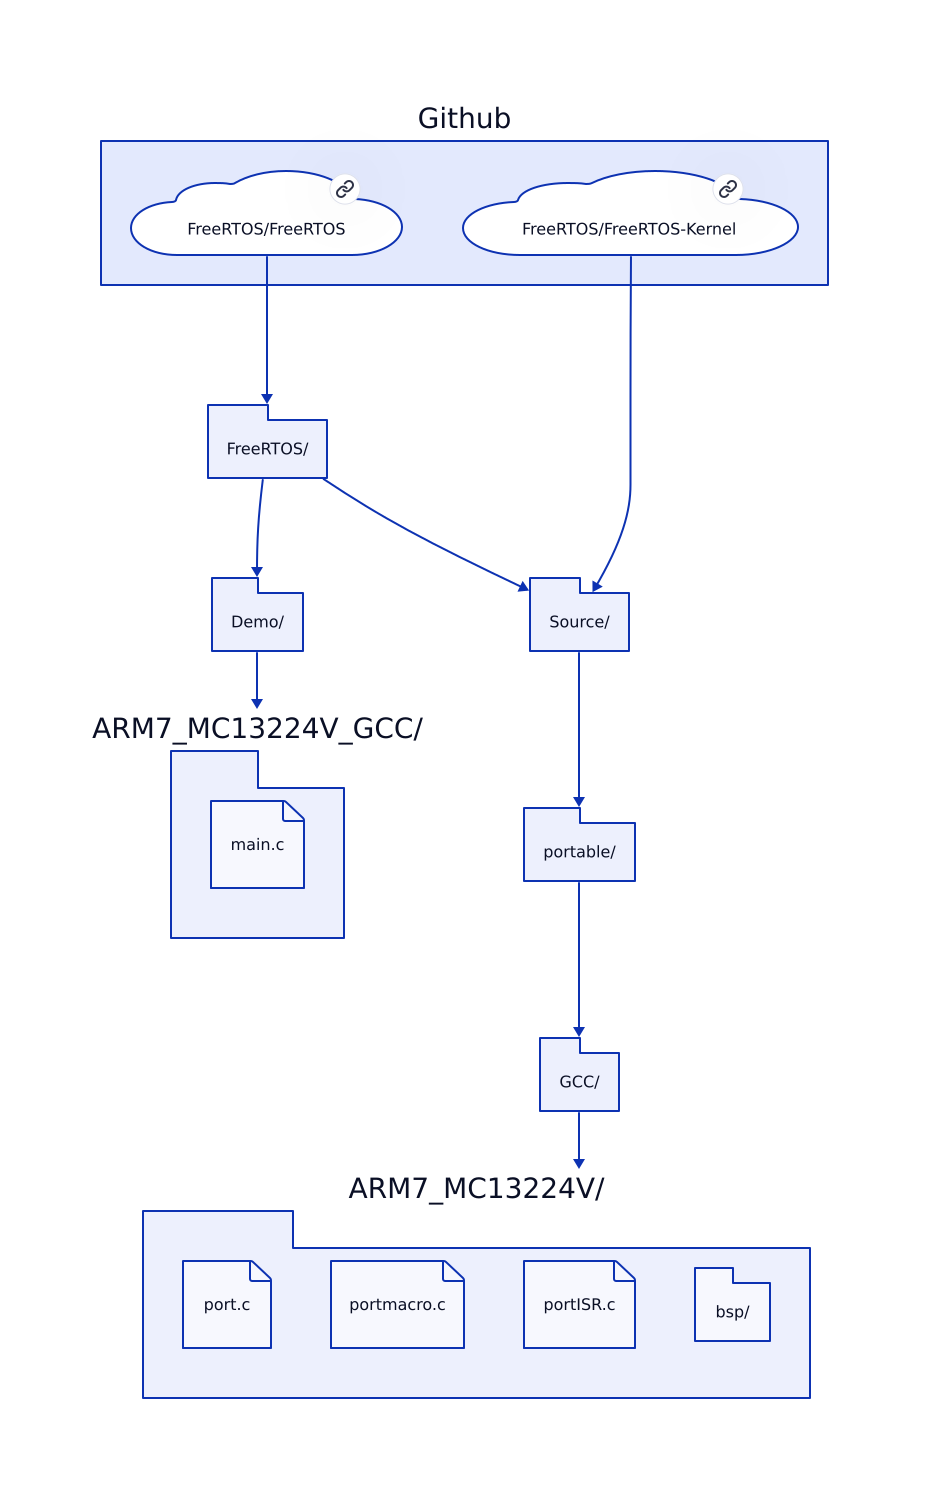
\includegraphics[width=\textwidth]{img/carpetasFreeRTOS.png}
\label{fig:DirsFreeRTOS}
\caption{Estructura de los directorios y archivos de FreeRTOS}
\end{figure}

\section{Paso 2: integración del BSP}
Antes de empezar a implementar dentro de FreeRTOS, decidí integrar el BSP dentro del port para que utilizar las herramientas que ya estaban implementadas en el BSP tango en el port como en la demo.
FreeRTOS utiliza una serie de \textit{Makefiles} para su compilación así que decidí sustituir el \textit{Makefile} del BSP por un \textit{CMakeLists.txt} y así poder incluir la compilación del BSP más orgánicamente en el port.

\section{Paso 3: Ampliación del BSP}
FreeRTOS requiere de interrupciones periódicas para medir el tiempo transcurrido.

\section{Paso 4: }



	% Presupuesto

	% Conclusiones
	\chapter{Conclusiones y trabajos futuros}
\section{Conclusiones}
en vaya fregao me he metido

\section{Trabajos futuros}
Sería interesante crear un bsp para una placa más moderna y realizar un port de FreeRTOS a esa placa.



	% Trabajos futuros


	
	\newpage
	\bibliography{bibliografia}
	\bibliographystyle{plain}
	
\end{document}

